\documentclass[11pt]{article}

\usepackage[utf8]{inputenc}
\usepackage[margin=2cm]{geometry} 
\usepackage{hyperref}
\usepackage{graphicx}
\usepackage{float}
\usepackage{caption}
\usepackage{longtable}
\usepackage{minted}
\usepackage{appendix}
\usepackage{xcolor}
\usepackage{subfig}
\usepackage{bookmark}
\usepackage{array}
\usepackage{multirow}
\usepackage{rotating}
\usepackage{placeins}

\setlength{\parskip}{1em}
\setlength{\parindent}{0pt}

\begin{document}

% ============ TITLE PAGE ============
\title{\huge Data Mining \& Machine Learning F20DL} 
% \\ {\small{\url{ }}}}
\author{Group 4\\Lewis Wilson, Sam Fay-Hunt, Kamil Szymczak, Chun Man }
\date{\today}
\maketitle

% ============ TABLE OF CONTENTS ============
\newpage
\tableofcontents
\thispagestyle{empty}
\pagebreak
\setcounter{page}{1}
% ============   ============   ============
\newpage
\section{Introduction}
We used Weights and Biases (\url{https://wandb.ai/home}) to run these experiments which allowed us to generate the graphs shown in this document.


\newpage
\section{Variation in performance with size of the training and testing sets}

\newpage
\section{Variation in performance with the change in the learning paradigm (Decision Trees versus
Neural Nets)}

\newpage
\section{Variation in performance with varying learning parameters in Decision Trees}

\subsection{J48}



\newpage
\subsection{Random Forest}

\begin{table}[ht]
  \centering
  \begin{tabular}{|p{0.25\linewidth} | p{0.7\linewidth}|} 
    \hline
    \textbf{Parameter}  & \textbf{Conclusion} \\ \hline
    max\_features & Contains the options "auto", "sqrt" and "log2". From (Figure \ref{RFAccOverTime}) we can see that "sqrt" has a higher accuracy overall, the accuracy of "log2" varies between the lower end and the median accuracy value.\\ \hline
    min\_samples\_split & The minimum samples required to split a node has very little impact on accuracy.  \\ \hline
    criterion & Gives a perfect negative correlation with respect to accuracy. Correlation values being [Gini = -0.404 ], [Entropy = 0.404 ]. \\ \hline
    n\_estimators & This is defined as the number of trees in the forest, it seems to have very little correlation but high importance. \\ \hline
    min\_samples\_leaf & Gives a strong negative correlation in terms of accuracy, meaning the higher minimum samples at a leaf node, the lower the accuracy. \\ \hline
    min\_weight\_fraction\_leaf & Has a somewhat positive correlation to accuracy. e.g. total weight required at a leaf node varies between 76\% and 89\% accuracy\\ \hline

  \end{tabular}
\end{table}\label{RF_Analysis_Table}
See Parameter Importance (Figure \ref{RF_ParamImp1})

\newpage
\section{Variation in performance with varying learning parameters in Neural Networks}
\subsection{Linear Classifier}



\newpage
\subsection{Multilayer Perceptron}

\begin{table}[ht]
  \centering
  \begin{tabular}{|p{0.25\linewidth} | p{0.7\linewidth}|} 
    \hline
    \textbf{Parameter}  & \textbf{Conclusion} \\ \hline
    alpha & This has a positive correlation to accuracy as higher alpha value equates to higher accuracy. \\ \hline 
    solver & lbfgs is the most accurate value of this parameter with a strong positive correlation out of the three (lbfgs, adam, sgd). \\ \hline
    max\_iter & The maximum number of iterations - In general, higher accuracy can be achieved with a larger amount of max iterations. \\ \hline
    activation & Out of the four activation functions (relu, tanh, identity and logistic), relu is the only one with a positive correlation, giving the highest accuracy overall. \\ \hline  
    learning\_rate & 'adaptive' achieves the highest accuracy while, 'constant' and 'invscaling' vary widely. \\ \hline  
    hidden\_layer\_sizes & Has a negative correlation - the number neurons in the n-th hidden layer has no effect on accuracy. \\ \hline
  \end{tabular}
\end{table}\label{MLP_Analysis_Table}

\newpage
\section{Variation in performance according to different metrics (TP Rate, FP Rate, Precision,
Recall, F Measure, ROC Area)}

% ============ APPENDICES BEGINNING ============
\pagebreak
\appendix
\appendixpage
\addappheadtotoc
\begin{appendices}

\section{Appendix A}

% =================== Workload Split Table ===================

\subsection{Workload split}
  
  \begin{table}[ht]
    \centering
    \begin{tabular}{|p{0.25\linewidth} | p{0.8\linewidth}|} 
      \hline
      \textbf{Team member}  & \textbf{Involvement} \\ \hline
      Lewis Wilson & text here \\ \hline
      Chun Man & text here  \\ \hline
      Sam Fay-Hunt & text here \\ \hline
      Kamil Szymczak & text here \\ \hline
    \end{tabular}
  \end{table}\label{ContributionTab}

As a team we are happy with everyone's contributions to the project. All team members were punctual and showed up to all scheduled meetings. Sam took the lead as project manager throughout the project delegating the workload and providing support to others.


% =================== J48 here ===================
\newpage
\section{J48}





\FloatBarrier
% =================== Random Forest here ===================
\newpage
\section{Random Forest}

\subsection{Random Forest Parameter Importance}
  \begin{table}[ht]
    \centering
    \begin{tabular}{|p{0.3\linewidth} | p{0.3\linewidth}| p{0.3\linewidth}|} 
      \hline
      \textbf{Parameter Config}  & \textbf{Importance} & \textbf{Correlation} \\ \hline
        min\_samples\_split & 0.005 & 0.306 \\ \hline
        min\_samples\_leaf & 0.375 & -0.725 \\ \hline
        n\_estimators & 0.016 & 0.092 \\ \hline
        min\_weight\_fraction\_leaf & 0.013 & 0.123 \\ \hline
    \end{tabular}
  \end{table}\label{RF_ParamImp1}

  \begin{table}[ht]
    \centering
    \begin{tabular}{|p{0.3\linewidth} | p{0.3\linewidth}| p{0.3\linewidth}|} 
      \hline
      \textbf{Parameter Config}  & \textbf{Importance} & \textbf{Correlation} \\ \hline
      max\_features.value\_sqrt & 0.001 & 0.563 \\ \hline
      max\_features.value\_log2 & 0.565 & -0.752 \\ \hline
      criterion.value\_entropy & 0.012 & 0.404 \\ \hline
      criterion.value\_gini & 0.012 & -0.404 \\ \hline
    \end{tabular}
  \end{table}\label{RF_ParamImp2}

\begin{sidewaysfigure}[h]
    \caption {Accuracy over time - Random Forest} \label{RFAccOverTime}
    \centering
    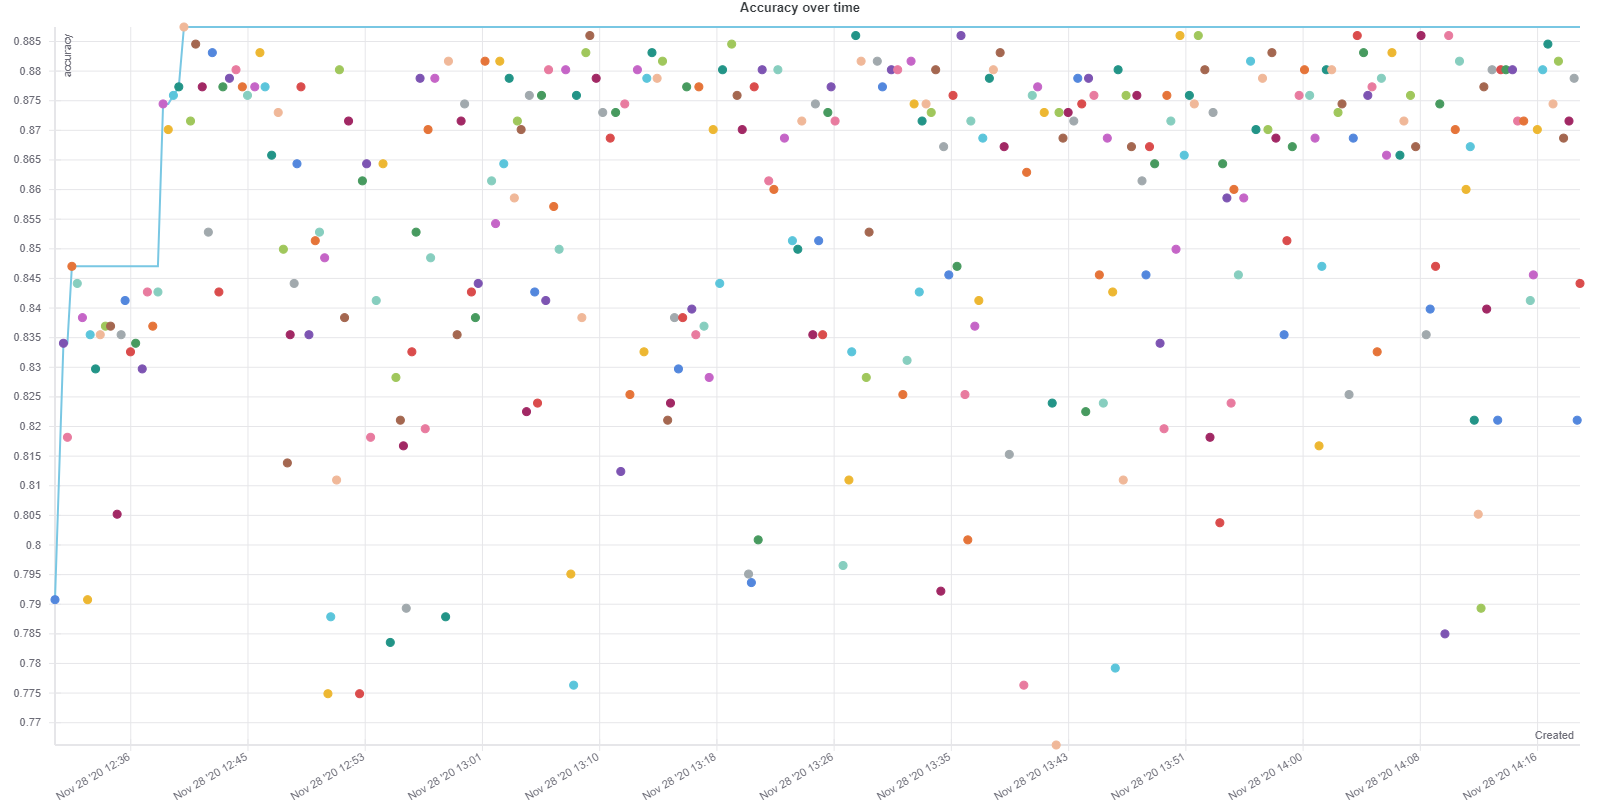
\includegraphics[width = \textwidth, height = \textwidth, keepaspectratio]{Images/RF Acc over time.png}
\end{sidewaysfigure}

\begin{sidewaysfigure}[h]
    \caption {Random Forest Parameters} \label{ParallelCoordRF}
    \centering 
    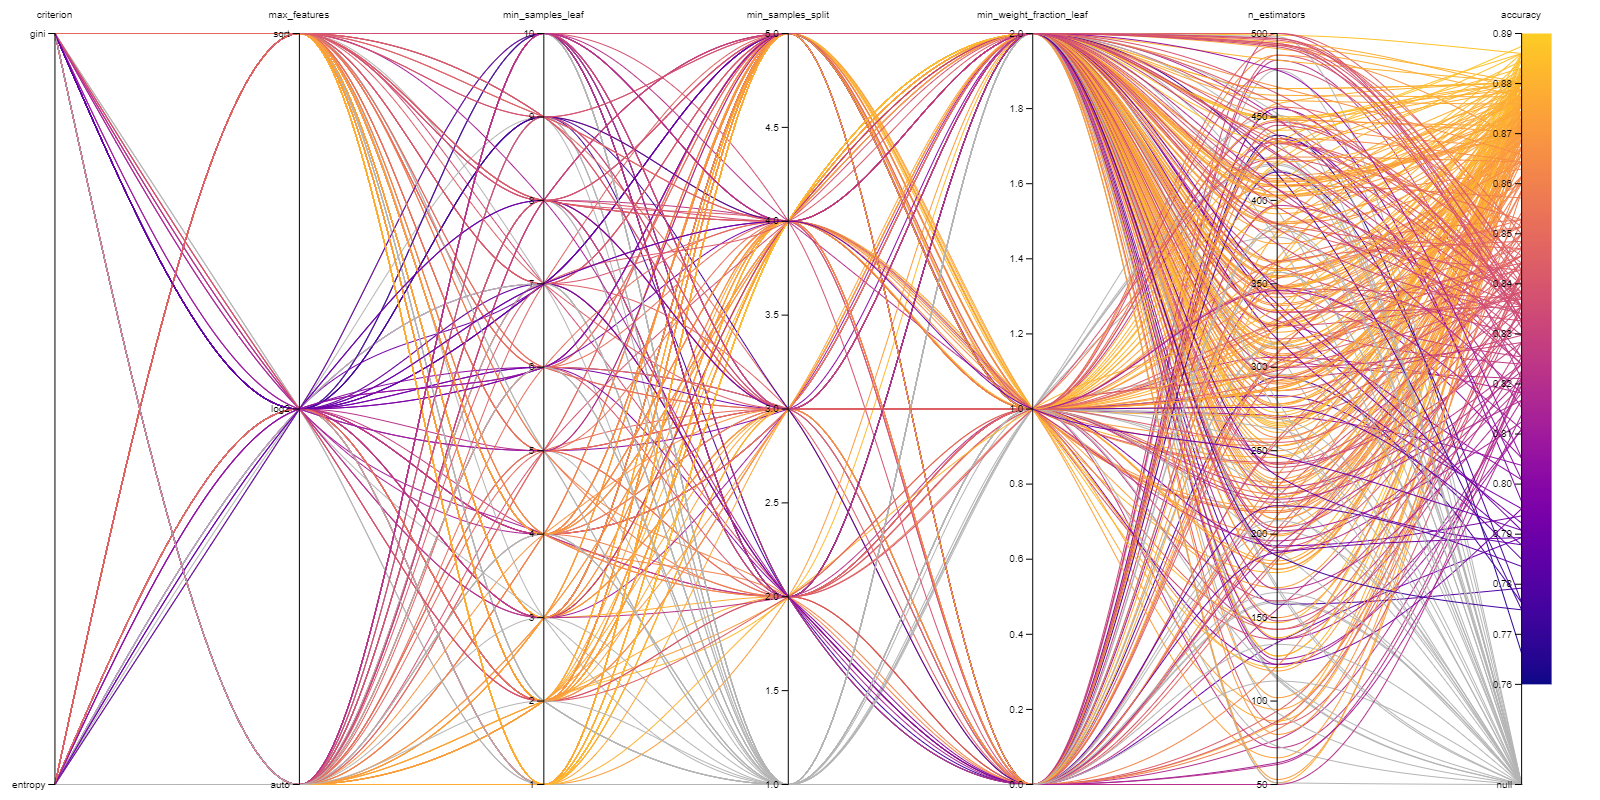
\includegraphics[width = \textwidth, height = \textwidth, keepaspectratio]{Images/RF ParallelCoordGraph.png}
\end{sidewaysfigure}


  
  \FloatBarrier
% =================== Linear Classifier here ===================
\newpage
\section{Linear Classifier}


\FloatBarrier
% =================== Multilayer Perceptron here ===================
\newpage
\section{Multilayer Perceptron}

\subsection{Multilayer Perceptron Parameter Importance}
  \begin{table}[ht]
    \centering
    \begin{tabular}{|p{0.3\linewidth} | p{0.3\linewidth}| p{0.3\linewidth}|} 
      \hline
      \textbf{Parameter Config}  & \textbf{Importance} & \textbf{Correlation} \\ \hline
        hidden\_layer\_sizes & 0.095 & -0.101 \\ \hline
        max\_iter & 0.091 & 0.072 \\ \hline
        alpha & 0.061 & 0.171 \\ \hline
    \end{tabular}
  \end{table}\label{MLP_ParamImp1}

  
  \begin{table}[ht]
    \centering
    \begin{tabular}{|p{0.3\linewidth} | p{0.3\linewidth}| p{0.3\linewidth}|} 
      \hline
      \textbf{Parameter Config}  & \textbf{Importance} & \textbf{Correlation} \\ \hline
        solver.value\_lbfgs & 0.530 & 0.728 \\ \hline
        solver.value\_adam & 0.027 & -0.245 \\ \hline
        solver.value\_sgd & 0.024 & -0.640 \\ \hline
        activation.value\_identity & 0.098 & -0.169 \\ \hline
        activation.value\_relu & 0.033 & 0.301 \\ \hline
        activation.value\_tanh & 0.018 & -0.035 \\ \hline
        activation.value\_logistic & 0.006 & -0.270 \\ \hline
        learning\_rate.value\_adaptive & 0.012 & 0.507 \\ \hline
        learning\_rate.value\_constant & 0.004 & -0.442 \\ \hline
        learning\_rate.value\_invscaling & 0.001 & -0.224 \\ \hline
    \end{tabular}
  \end{table}\label{MLP_ParamImp2}

\begin{sidewaysfigure}[h!]
    \caption {Accuracy over time - Multilayer Perceptron} \label{MLPAccOverTime}
    \centering
    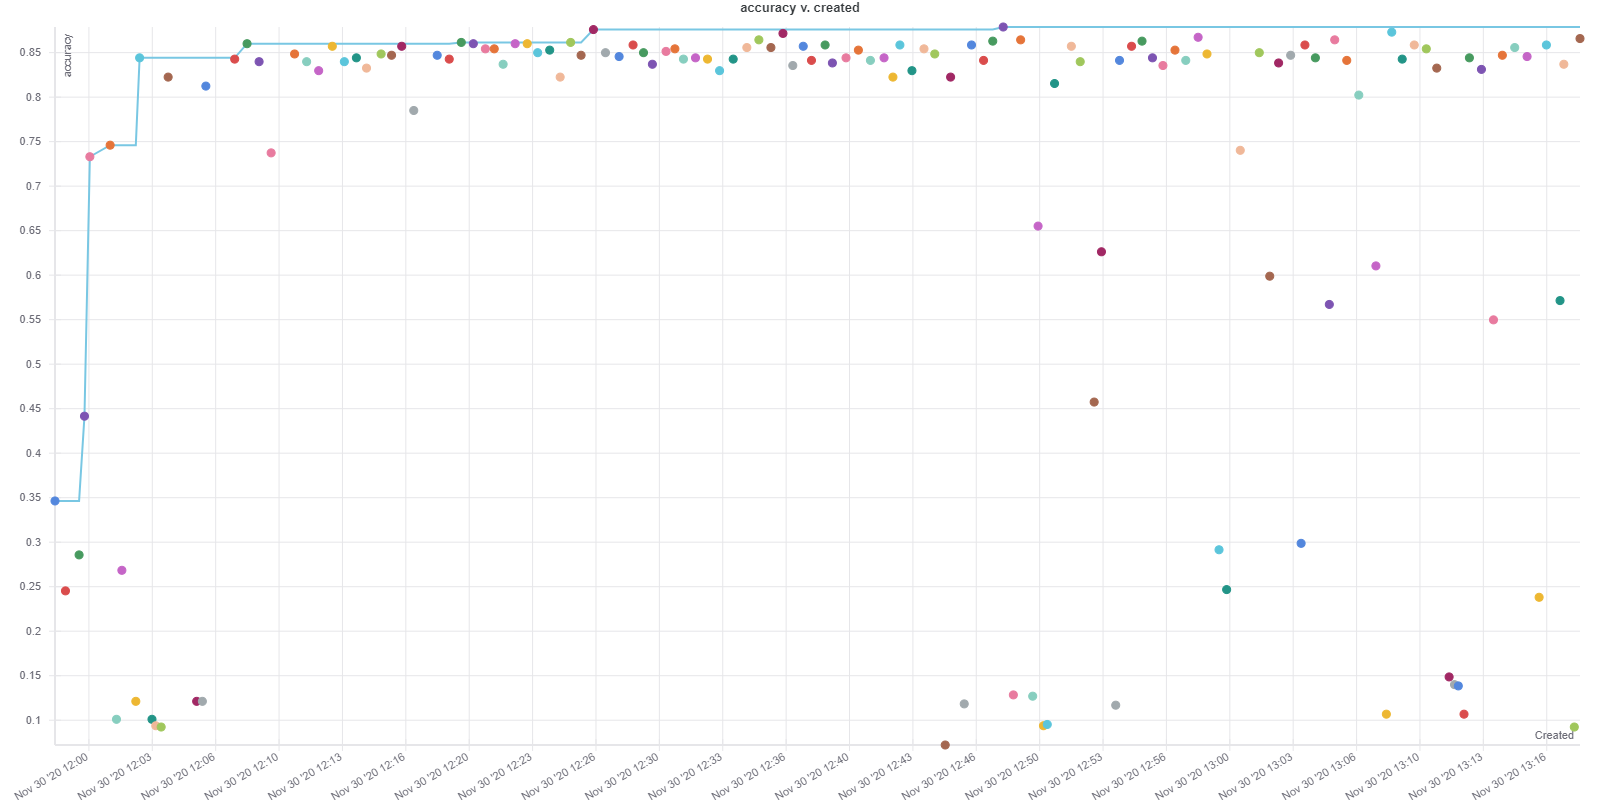
\includegraphics[width = \textwidth, height = \textwidth, keepaspectratio]{Images/MLP Acc over time.png}
\end{sidewaysfigure}

\begin{sidewaysfigure}[h]
  \caption {Multilayer Perceptron Parameters} \label{ParallelCoordMLP}
  \centering 
  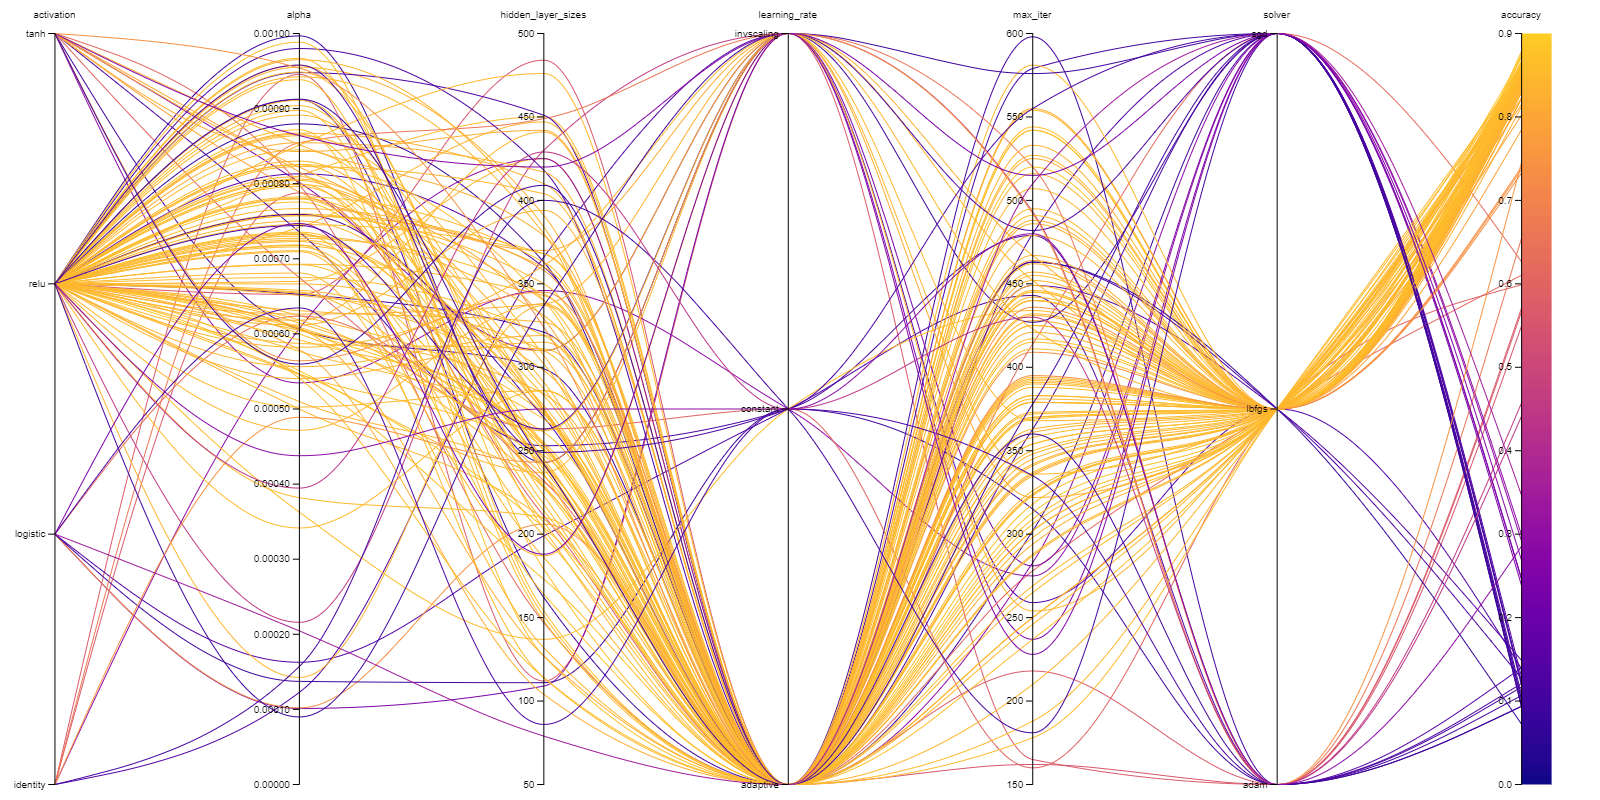
\includegraphics[width = \textwidth, height = \textwidth, keepaspectratio]{Images/MLP ParallelCoordGraph.png}
\end{sidewaysfigure}

\FloatBarrier
% =================== END APPENDIX ===================
\end{appendices}

\end{document}